\chapter{Contexte du stage}

\section{Le laboratoire ICube}

Le laboratoire \gls{icube} \cite{noauthor_icube_nodate}, organisme d'accueil de ce stage, est une unité de recherche de ce type. Fondé en 2013 à Strasbourg, il est le fruit d'une collaboration entre le \gls{cnrs}, l'\gls{unistra}, l'\gls{engees} et l'\gls{insa}. Environ 650 personnes y travaillent quotidiennement, principalement dans le domaine de la santé, l'environnement et le développement durable.

Le laboratoire est structuré en 17 équipes de recherche, réparties en quatre départements, et s’appuie sur sept plateformes technologiques (voir Figure \ref{fig:orga-icube}).

\begin{figure}[H]
\centering
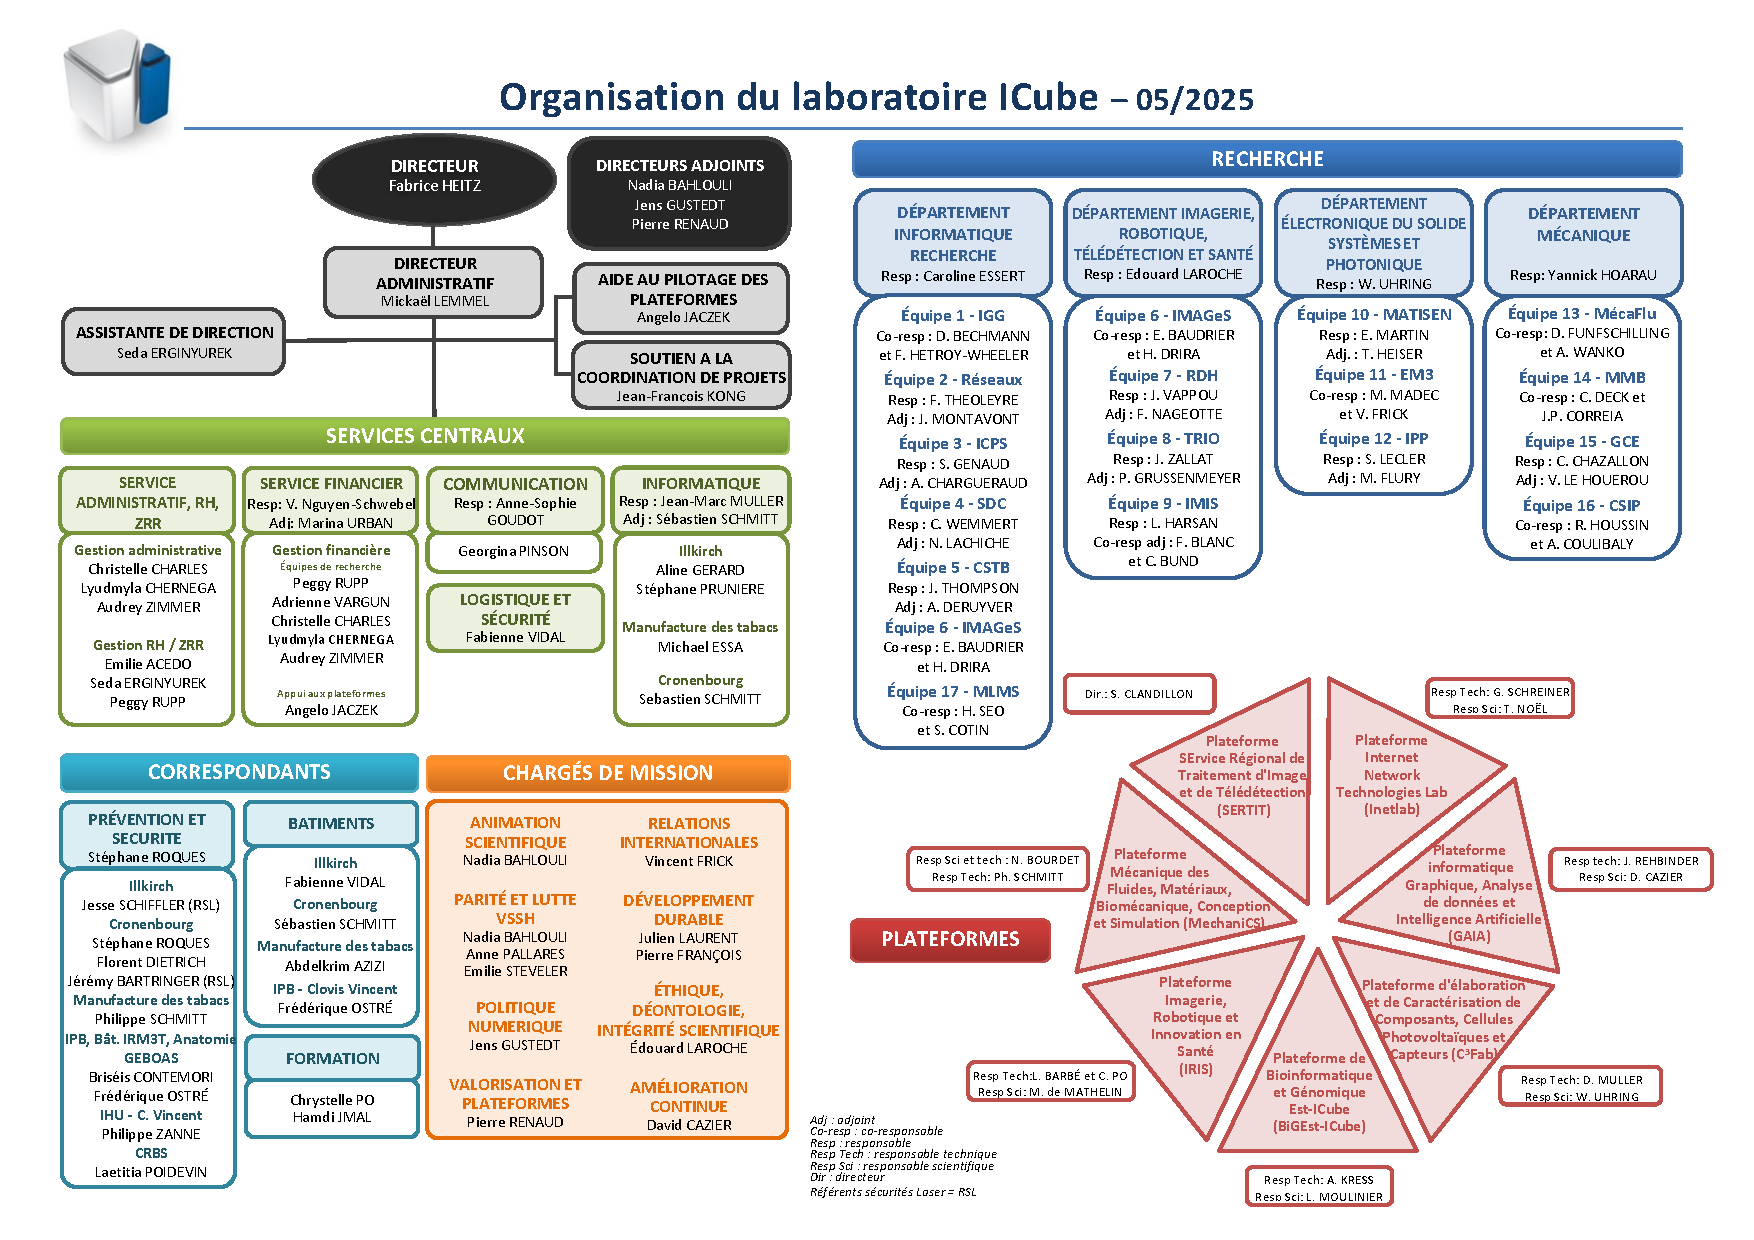
\includegraphics[width=\textwidth,page=1]{7-Contexte/pic/icube_organigramme.pdf}
\caption{Organisation du laboratoire \gls{icube}.}
\label{fig:orga-icube}
\end{figure}

Le stage s’est déroulé au sein de l’équipe \gls{rdh}, dont les recherches s’articulent autour de trois axes :
\begin{itemize}
\item \textbf{robotique médicale et imagerie interventionnelle} : développement de dispositifs et méthodes pour l’assistance aux procédures mini-invasives ;
\item \textbf{apprentissage, modélisation et science des données} : simulation biomécanique, mesures, génération et exploitation de données pour l’\gls{IA} ;
\item \textbf{systèmes complexes} : conception et commande mécatronique avancées de robots.
\end{itemize}

L’intégralité du stage s’est déroulée à l’INSA Strasbourg, dans la salle L1.14, équipée d’un système de capture de mouvement, dont l’utilisation sera détaillée plus loin.

\section{Contexte social et organisationnel}

Le statut de laboratoire public confère à ICube un mode de fonctionnement distinct de celui d’une entreprise privée : les résultats attendus relèvent avant tout de la production scientifique (publications, brevets, collaborations, formation de doctorants), plutôt que de critères financiers \cite{noauthor_laboratoire_2025}.

\subsection{Composition du personnel}

Les 650 membres se répartissent en plusieurs catégories :
\begin{itemize}
\item \textbf{chercheurs et enseignants-chercheurs}, permanents, assurant recherche et enseignement ;
\item \textbf{doctorants}, préparant une thèse dans les équipes ;
\item \textbf{post-doctorants}, recrutés sur projets ;
\item \textbf{ingénieurs et techniciens}, responsables du soutien expérimental et informatique ;
\item \textbf{personnel administratif}, en charge de la gestion et du support ;
\item \textbf{stagiaires}, souvent étudiants en master, intégrés ponctuellement aux projets.
\end{itemize}


Les chercheurs et enseignants-chercheurs disposent généralement d’un doctorat. La formation continue fait partie intégrante de leur métier : elle passe par la veille scientifique, la participation à des séminaires, conférences, ou encore à des écoles d’été.

\subsection{Conditions de travail}
Le fonctionnement repose sur une organisation souple : horaires flexibles, autonomie des équipes, congés gérés selon les règles de la fonction publique. Pour les stagiaires, les modalités sont avec le tuteur. Pour ma part, le stage s'est déroulé du 3 mars au 5 septembre 2025, à temps plein, incluant deux semaines de congés du 28 juillet au 8 août. Mes horaires étaient généralement de 8h30 à 17h, avec une pause déjeuner d'une heure et demie. Le télétravail était également possible lorsque l'accès au matériel n'était pas nécessaire, notamment pour l'étude bibliographique ou la rédaction du rapport.



%\paragraph{Cadre scientifique élargi}
%Le projet se rattache au domaine des robots modulaires reconfigurables et de la robotique d'essaim. Ces approches visent l'adaptabilité (ajuster morphologie ou topologie selon la tâche : port de charge, précision, accessibilité), la résilience (redistribution des rôles après perte ou défaillance d'un module), la scalabilité (ajout ou retrait d'unités sans ré‑ingénierie lourde) et la mutualisation (standardisation d'une unité de base pour réduire coûts de fabrication et de maintenance). Le recours temporaire à une plateforme terrestre holonome plutôt qu'aérienne permet un cycle expérimental rapide, une réduction du risque matériel et une collecte de données facilitée pour l'analyse des lois de commande distribuées.
%Le projet mobilise principalement l'axe systèmes complexes (modélisation cinématique et dynamique, synthèse de lois de commande distribuées) et l'axe apprentissage / données (instrumentation, exploitation de traces pour calibration et optimisation), tout en ouvrant des synergies vers des méthodologies transférables à des dispositifs multi‑modules (potentiel en robotique médicale ou architectures hybrides). Ce positionnement fournit un terrain intermédiaire avant transposition sur la plateforme aérienne initiale, tout en générant des connaissances sur la robustesse et la reconfiguration structurelle.
